\chapter[Resultados]{Resultados}
\label{ch:resultados}

Este Capítulo apresenta os resultados dos experimentos realizados no período de treino (2000--2020), validação (2021--2022) e teste (2023--2024), sobre os dados diários do S\&P~500. Os resultados são apresentados, mas serão discutidos e interpretados no Capítulo~\ref{ch:discussao}.

\section{Ablation Study: Variantes de Pré-processamento da LSTM}
\label{sec:res_ablation}

O \textit{ablation study} avaliou seis variantes de pré-processamento aplicadas à LSTM para determinar a combinação de entrada e normalização com melhor desempenho direcional. As variantes diferem no tipo de entrada (\textit{Close} bruto, \textit{Close} DWT \textit{denoised} ou Log-retornos DWT \textit{denoised}) e no tipo de normalização (Z-score ou Min-Max), conforme definido na Metodologia.

A Tabela~\ref{tab:variantes} apresenta as métricas de classificação direcional no conjunto de teste (período 2023--2024), ordenadas pelo \textit{Matthews Correlation Coefficient} (MCC) decrescente. São incluídas as acurácias (Acc.) de treino, validação e teste para análise de generalização, área sob a curva ROC (AUC), além do valor do Teste de McNemar ($p < 0{,}05$ rejeição da hipótese nula).

\begin{landscape}
\begin{table}[H]
\centering
\caption{Resultados \textit{Ablation study} da LSTM.}
\label{tab:variantes}
\small
\begin{tabular}{@{}clccccccccc@{}}
\toprule
\textbf{Var.} & \textbf{Entrada} & \textbf{Norm.} & \textbf{Acc Treino (\%)} & \textbf{Acc Val (\%)} & \textbf{Acc Teste (\%)} & \textbf{F1 (\%)} & \textbf{MCC} & \textbf{AUC} & \textbf{McNemar $p$} & \textbf{Ép.} \\
\midrule
B & \textit{Close} DWT  & Z-score  & 68{,}3 & 68{,}6 & \textbf{67,5} & \textbf{72,0} & \textbf{0,333} & \textbf{0,724} & $<$0,001 & 25 \\
F & \textit{Close} DWT  & Min-Max  & 65{,}9 & 65{,}2 & 64{,}7 & 70{,}2 & 0{,}273 & 0{,}687 & 0,004 & 42 \\
D & LogRet DWT         & Z-score  & 66{,}9 & 65{,}4 & 62{,}3 & 70{,}8 & 0{,}211 & 0{,}671 & 0,017 & 19 \\
A & \textit{Close} bruto & Z-score & 67{,}8 & 62{,}6 & 61{,}5 & 69{,}6 & 0{,}195 & 0{,}652 & 0,049 & 21 \\
C & Log-retornos        & Z-score  & 67{,}8 & 62{,}6 & 61{,}5 & 69{,}6 & 0{,}195 & 0{,}652 & 0,049 & 21 \\
E & \textit{Close} bruto & Min-Max & 55{,}3 & 54{,}5 & 56{,}5 & 72{,}2 & 0{,}000 & 0{,}512 & 1,000 & 11 \\
\bottomrule
\end{tabular}
\end{table}
\end{landscape}

Os gráficos da Figura~\ref{fig:comparativo_variantes} ilustram as métricas de teste (Acurácia, F1, AUC e MCC) representadas na Tabela \ref{tab:variantes} para as seis variantes. A Figura~\ref{fig:overfitting_variantes} mostra as curvas de perda de treino e validação por variante ao longo das épocas de treinamento, com o marcador indicando o ponto de melhor validação (menor BCE Loss de validação) restaurado pelo \textit{early stopping}. A Figura~\ref{fig:probabilidades_variantes} apresenta os histogramas com as frequências que as probabilidades $P(\textit{sobe}) \in [0,1]$ resultaram no resultado real (sobe/desce), por cada variante no conjunto de teste. Os histogramas representam a classe/valor real por cores (sobe = verde, desce = vermelho), e um modelo discriminativo exibe distribuições claramente separadas, porém com uma tendência de concentrar a maior parte dos erros em torno de 0.5 (mancha escura que indica ambas as cores sobrepostas), onde a previsão possui uma maior incerteza. Para casos de modelos degenerados, como a variante E, as probabilidades são concentradas em torno de um único valor, indicando que a previsão é quase sempre a mesma e não está baseada em padrões do mercado.

\begin{figure}[H]
    \centering
    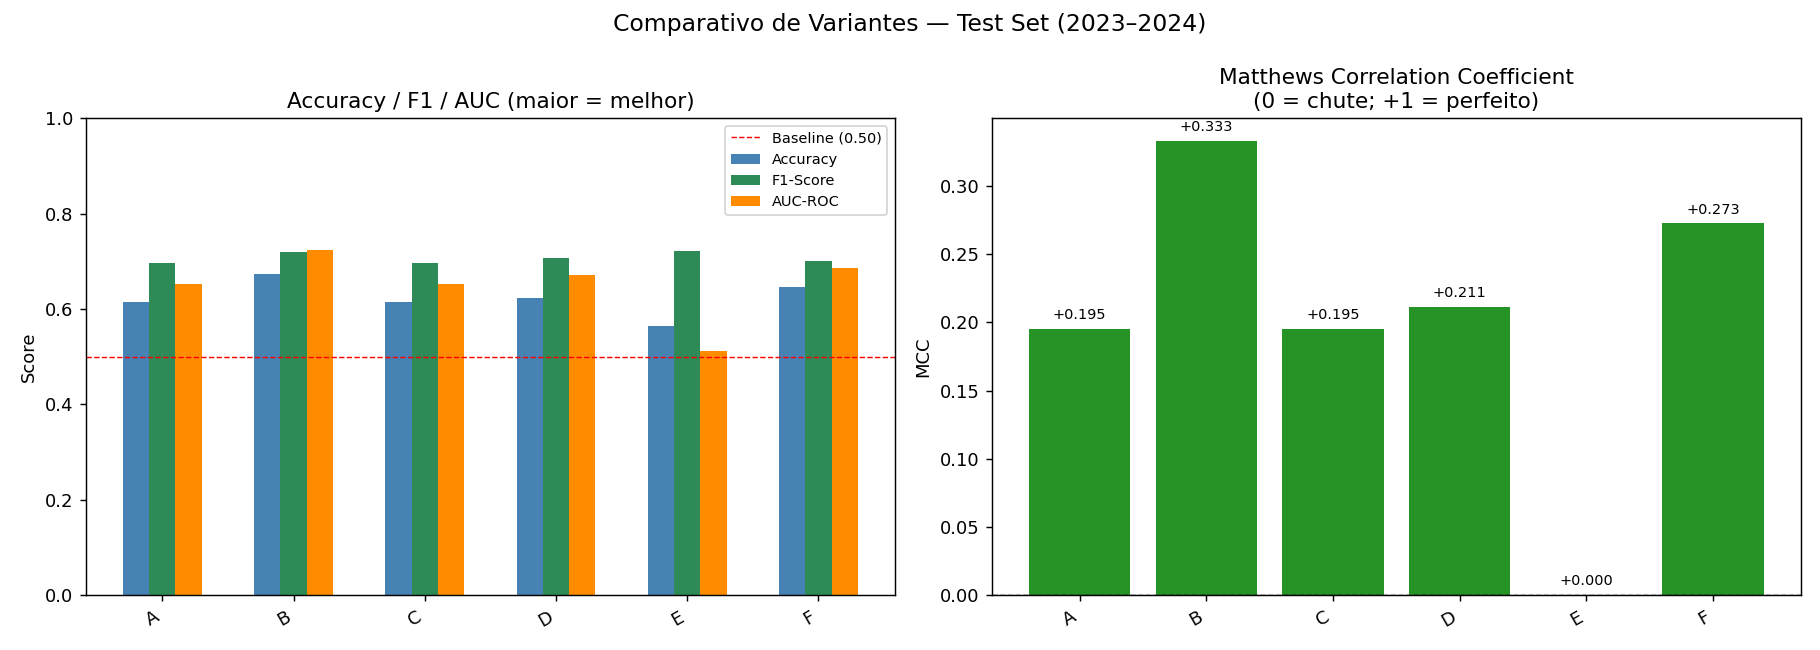
\includegraphics[width=\textwidth]{figuras/comparativo_variantes.png}
    \caption{Métricas de classificação direcional no teste por variante do \textit{ablation study}.}
    \label{fig:comparativo_variantes}
\end{figure}

\begin{figure}[H]
    \centering
    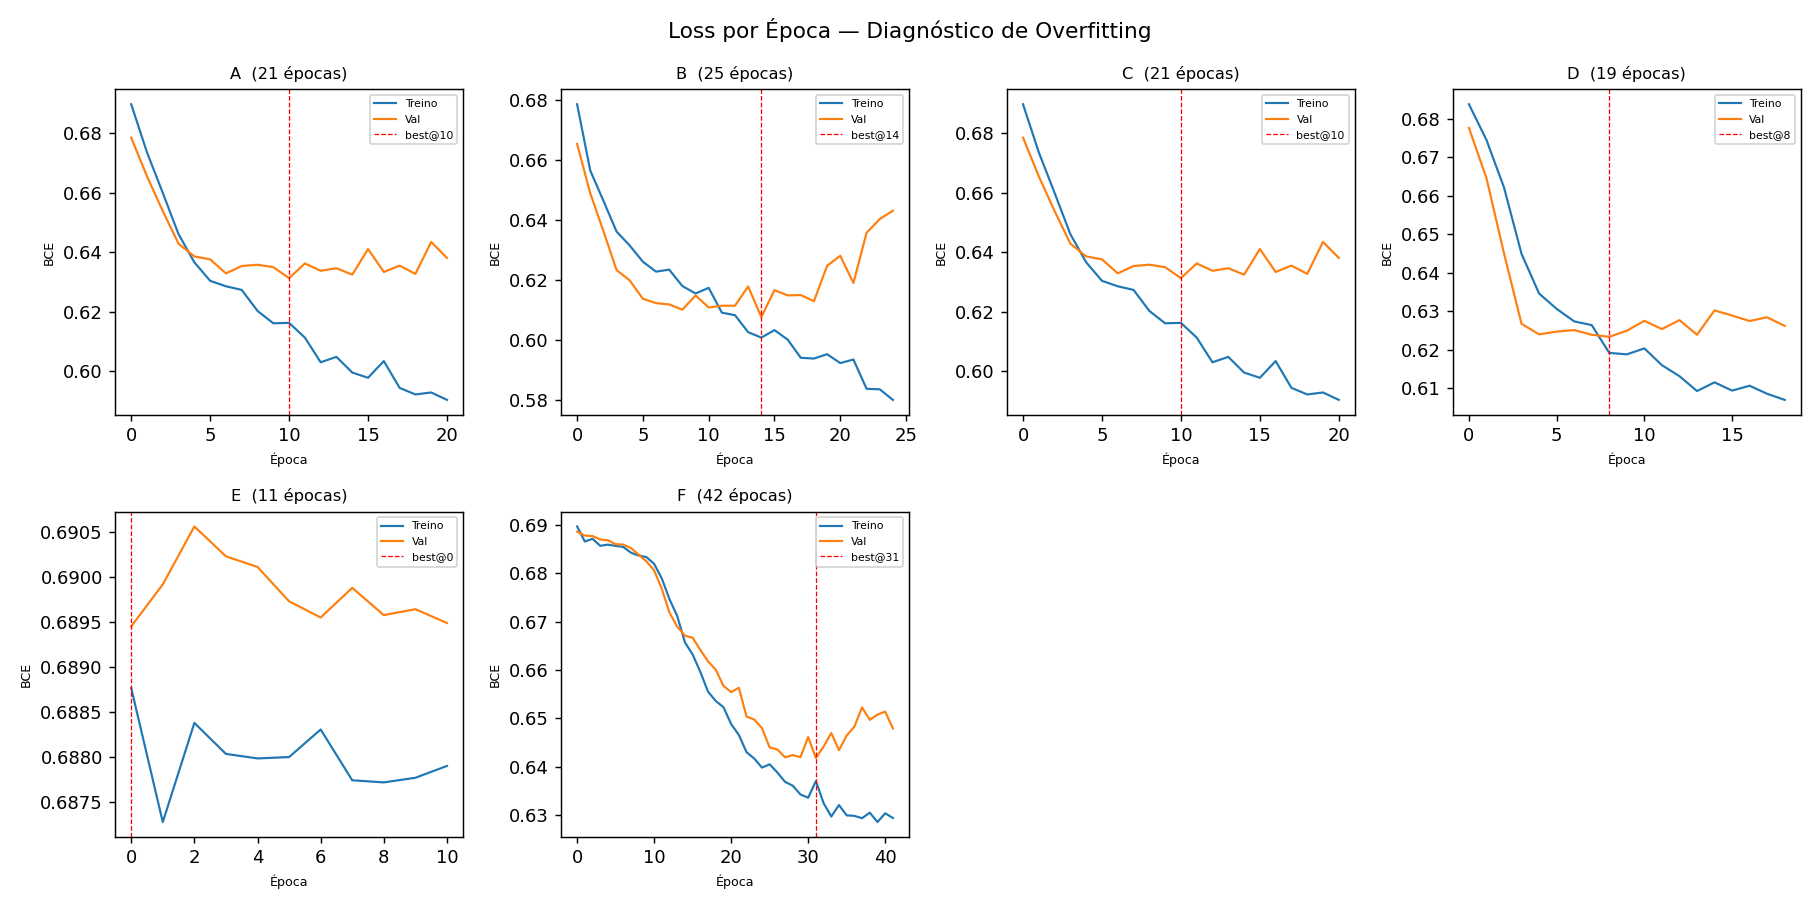
\includegraphics[width=\textwidth]{figuras/overfitting_variantes.png}
    \caption{Curvas de perda de treino e validação por época para cada variante.}
    \label{fig:overfitting_variantes}
\end{figure}

\begin{figure}[H]
    \centering
    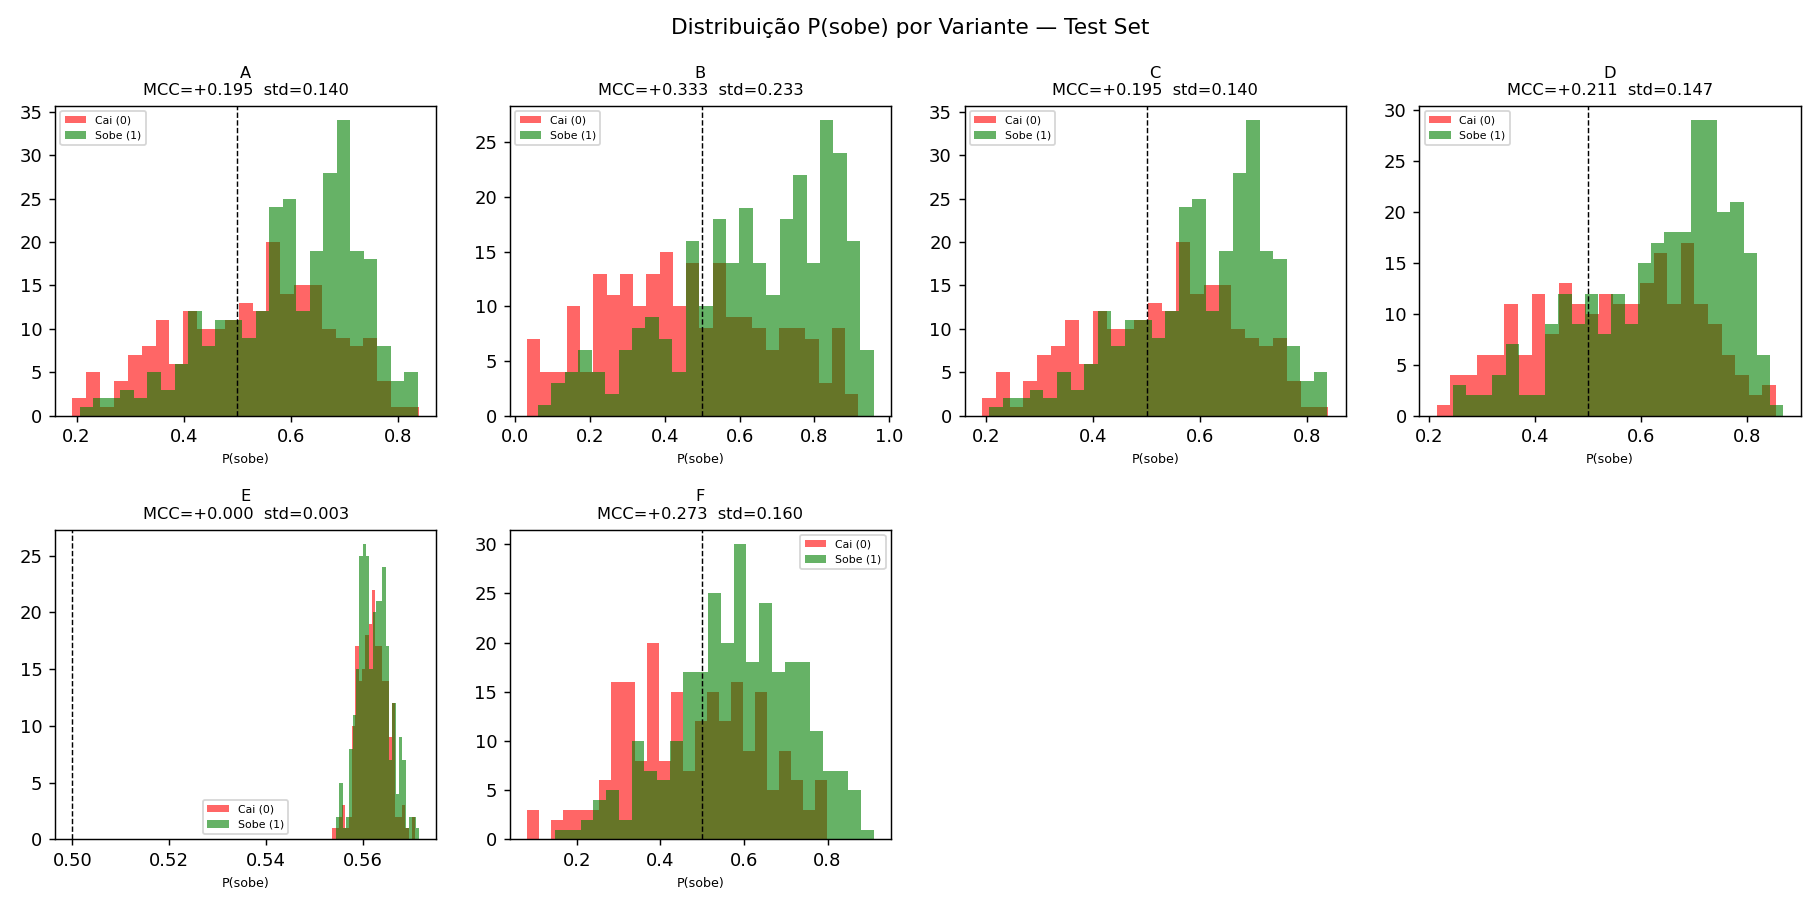
\includegraphics[width=\textwidth]{figuras/probabilidades_variantes.png}
    \caption{Distribuição de $P(\textit{sobe})$ no conjunto de teste por variante e classe/valor real.}
    \label{fig:probabilidades_variantes}
\end{figure}

A Figura~\ref{fig:resultados_B} detalha os resultados da variante B (LSTM com \textit{Close} DWT + Z-score), a variante que obteve o maior MCC no \textit{ablation study}. O gráfico do painel superior esquerdo indica a série do S\&P~500 no período de teste (2023--2024) com marcação de acertos (verde) e erros (vermelho) de prever a direção (sobe/desce). Os painéis da direita repetem os resultados das Figuras \ref{fig:overfitting_variantes} e \ref{fig:probabilidades_variantes} para a variante B, enquanto o painel inferior esquerdo apresenta a curva ROC calculada (AUC = 0,724).

\begin{figure}[H]
    \centering
    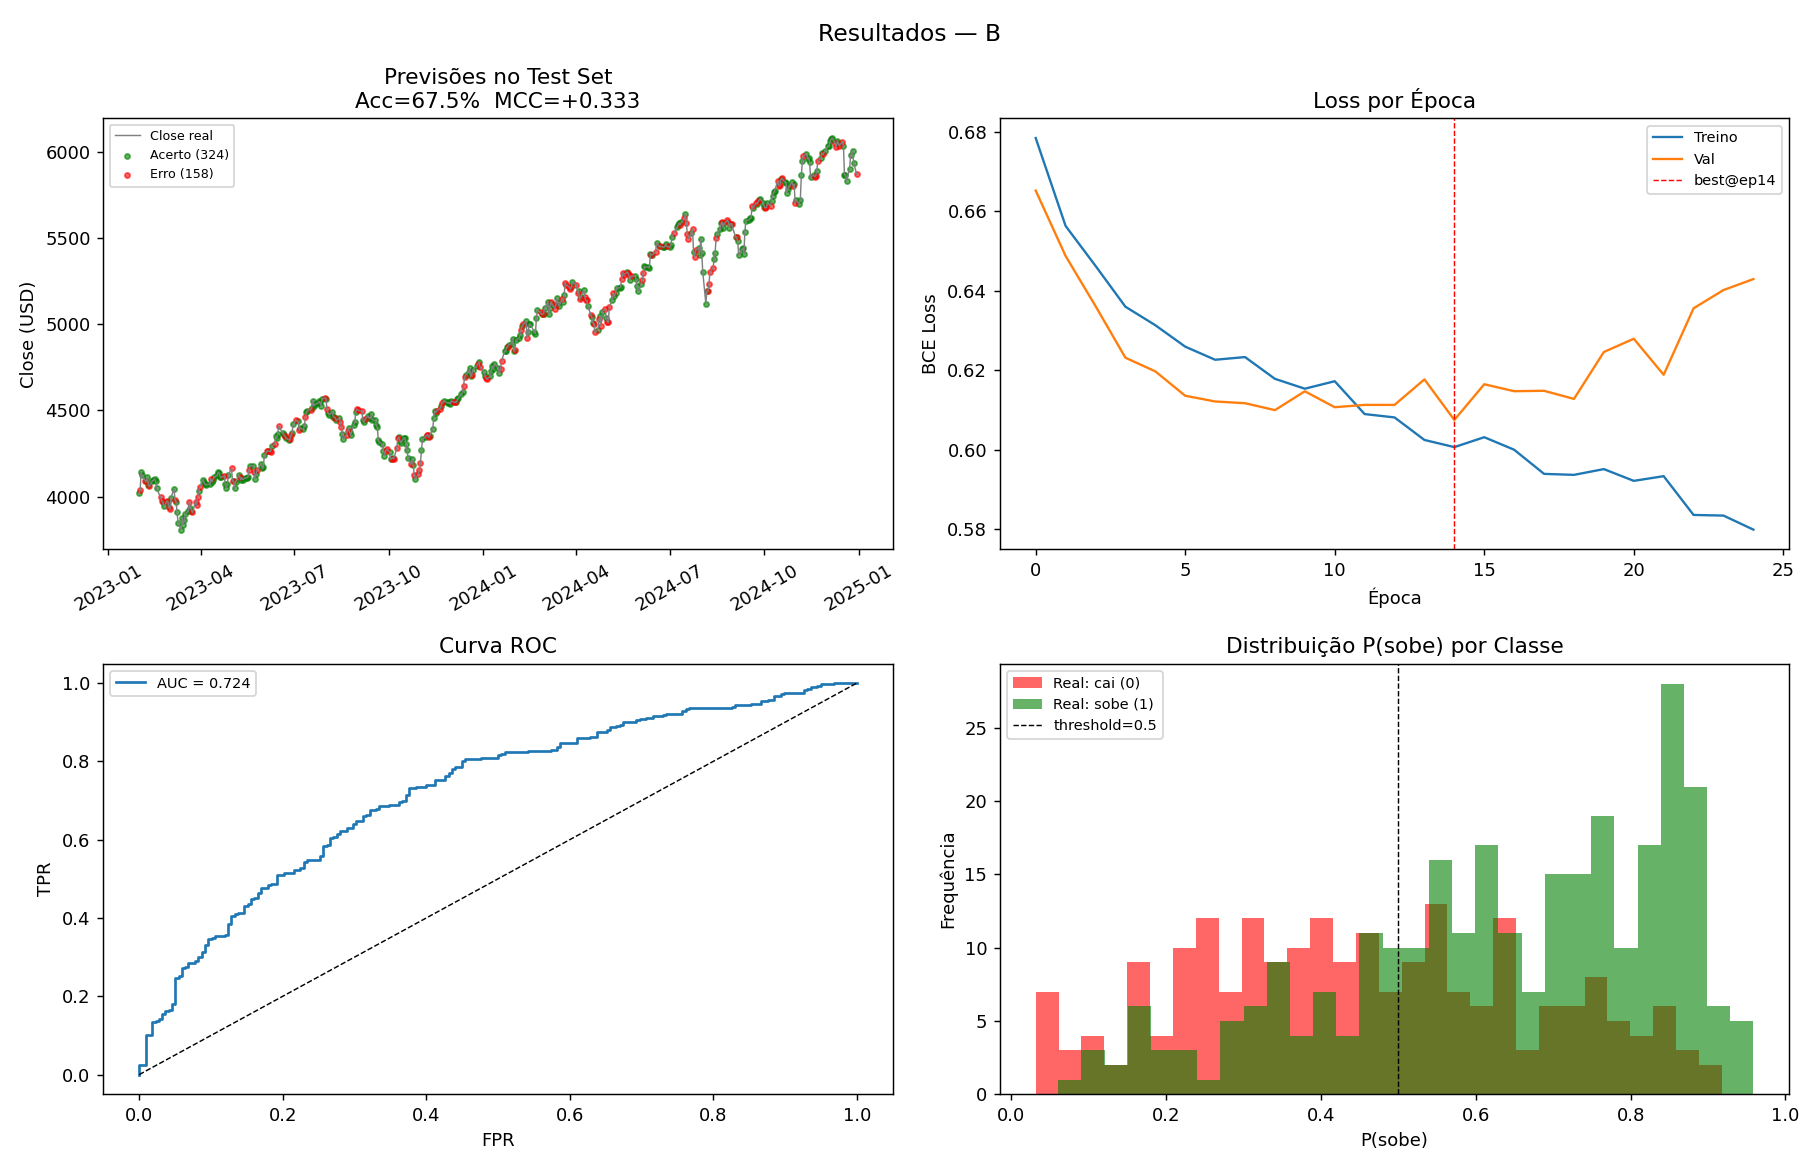
\includegraphics[width=\textwidth]{figuras/resultados_B.png}
    \caption{Resultados da variante~B.}
    \label{fig:resultados_B}
\end{figure}

\section{Modelos SOTA: xLSTM-TS e Transformer-TS}
\label{sec:res_sota}

Os modelos xLSTM-TS e Transformer-TS foram aplicados ao S\&P~500 com o mesmo período de tempo do \textit{ablation study} (200--2024), recebendo como entrada apenas o \textit{Close} com pré processamento DWT causal \& Min-Max fit-treino e com janela de 150 dias. Ambos foram treinados para regressão, permitindo comparação direta entre as duas arquiteturas. A direção prevista foi derivada em pós-processamento pela diferença entre previsões consecutivas.  

As Tabelas~\ref{tab:xlstm_metricas} e~\ref{tab:transformer_metricas} apresentam as métricas obtidas: de regressão (MAE, RMSE, RMSSE, MAPE e $R^2$); e direcionais derivadas (Acurácia, Recall, Precisão por classe e F1) para o conjunto de teste de cada modelo.

\begin{table}[H]
\centering
\caption{Métricas de regressão e direção do xLSTM-TS no conjunto de teste (2023--2024).}
\label{tab:xlstm_metricas}
\begin{tabular}{@{}llr@{}}
\toprule
\textbf{Categoria} & \textbf{Métrica} & \textbf{Valor} \\
\midrule
\multirow{5}{*}{Regressão} 
 & MAE   & 235,80 USD \\
 & RMSE  & 375,40 USD \\
 & RMSSE & 16,06 \\
 & MAPE  & 4,26\% \\
 & $R^2$ & 0,662 \\
\midrule
\multirow{5}{*}{Direcional (derivada)}
 & Acurácia          & 75,8\% \\
 & Recall            & 76,6\% \\
 & Precisão (sobe)   & 83,3\% \\
 & Precisão (desce)  & 65,7\% \\
 & F1                & 79,8\% \\
\bottomrule
\end{tabular}
\end{table}

\begin{table}[H]
\centering
\caption{Métricas de regressão e direcionais do Transformer-TS no conjunto de teste (2023--2024).}
\label{tab:transformer_metricas}
\begin{tabular}{@{}llr@{}}
\toprule
\textbf{Categoria} & \textbf{Métrica} & \textbf{Valor} \\
\midrule
\multirow{5}{*}{Regressão}
 & MAE   & 541,81 USD \\
 & RMSE  & 706,64 USD \\
 & RMSSE & 30,23 \\
 & MAPE  & 10,19\% \\
 & $R^2$ & $-$0,20 \\
\midrule
\multirow{5}{*}{Direcional (derivada)}
 & Acurácia          & 75,6\% \\
 & Recall            & 86,9\% \\
 & Precisão (sobe)   & 77,0\% \\
 & Precisão (desce)  & 72,3\% \\
 & F1                & 81,6\% \\
\bottomrule
\end{tabular}
\end{table}

As Figuras~\ref{fig:xlstm_resultados} e~\ref{fig:transformer_resultados} exibem quatro painéis para análise dos resultados de cada modelo, ambas com o mesmo layout. Painel superior esquerdo: Previsões no conjunto de teste; série real S\&P~500 (linha azul escuro) e a série prevista pelo modelo (linha cinza tracejada), ao longo de 2023–2024; cada dia é marcado com um ponto verde (direção derivada acertada) ou vermelho (direção derivada errada). Painel superior direito: curvas de perda MSE (normalizada) de treino e validação até o \textit{early stopping}. O xLSTM-TS convergiu em 103 épocas (melhor validação na época 63) e o Transformer-TS em 63 épocas (melhor validação na época 23). Painel inferior esquerdo: \textit{Scatter} Real vs Previsto; a linha tracejada representa previsão perfeita, onde o valor previsto (eixo X) coincide exatamente com o valor real (eixo Y). Painel inferior direito: frequência dos erros absolutos de previsão, em USD, ao longo do período de teste e indicação da média desses erros (MAE = 235,80 USD para o xLSTM-TS e MAE = 541,81 USD para o Transformer-TS).

\begin{figure}[H]
    \centering
    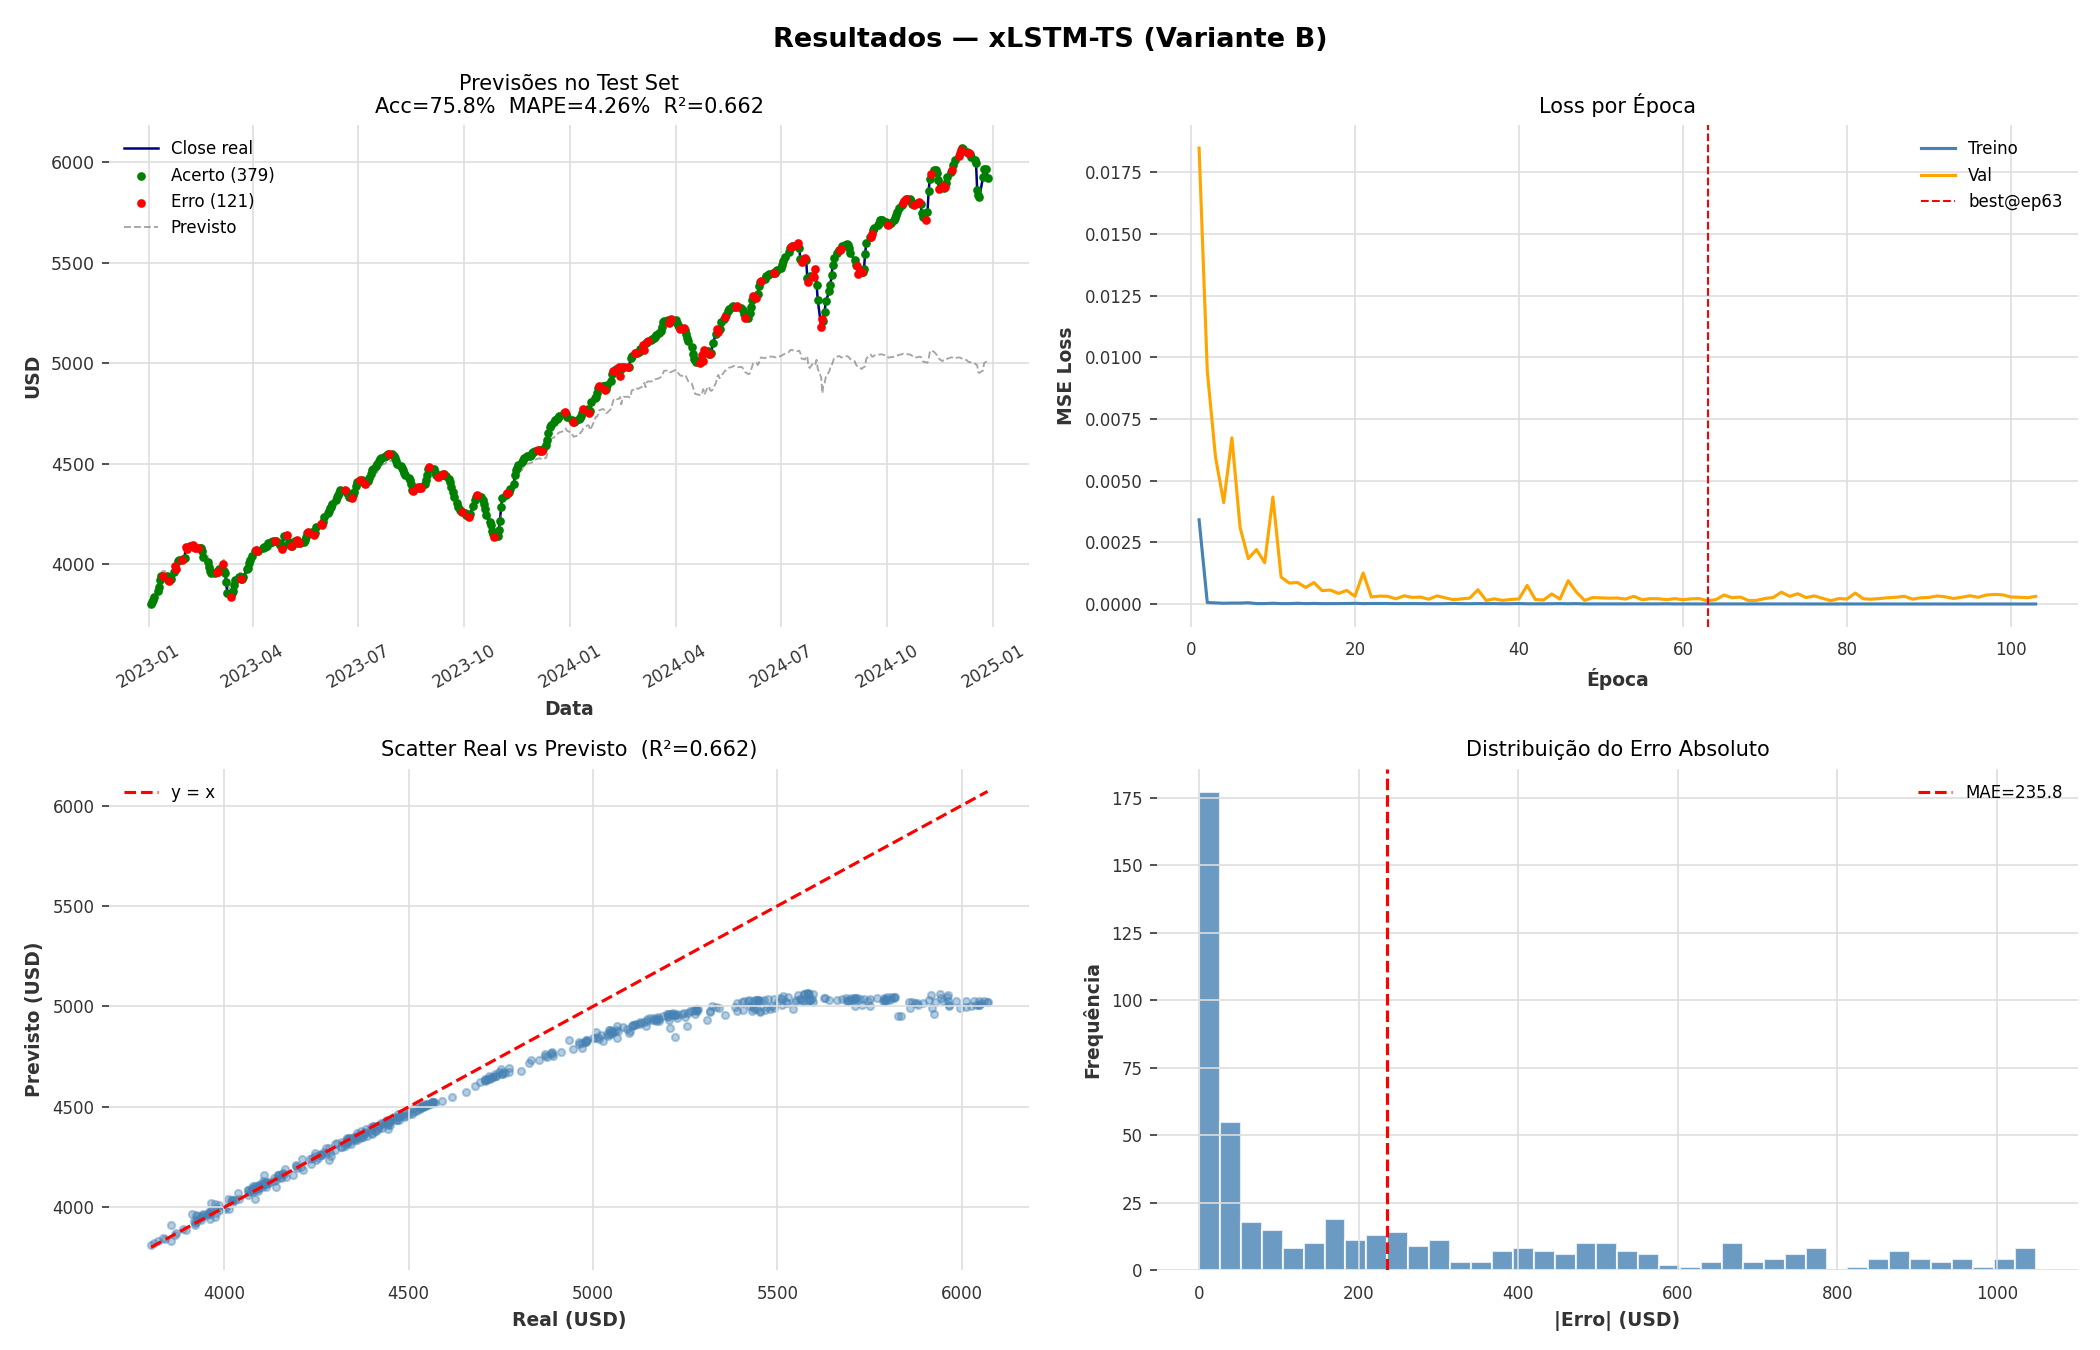
\includegraphics[width=\textwidth]{figuras/xlstm_ts_resultados.png}
    \caption{Resultados do xLSTM-TS no conjunto de teste (2023--2024).}
    \label{fig:xlstm_resultados}
\end{figure}

\begin{figure}[H]
    \centering
    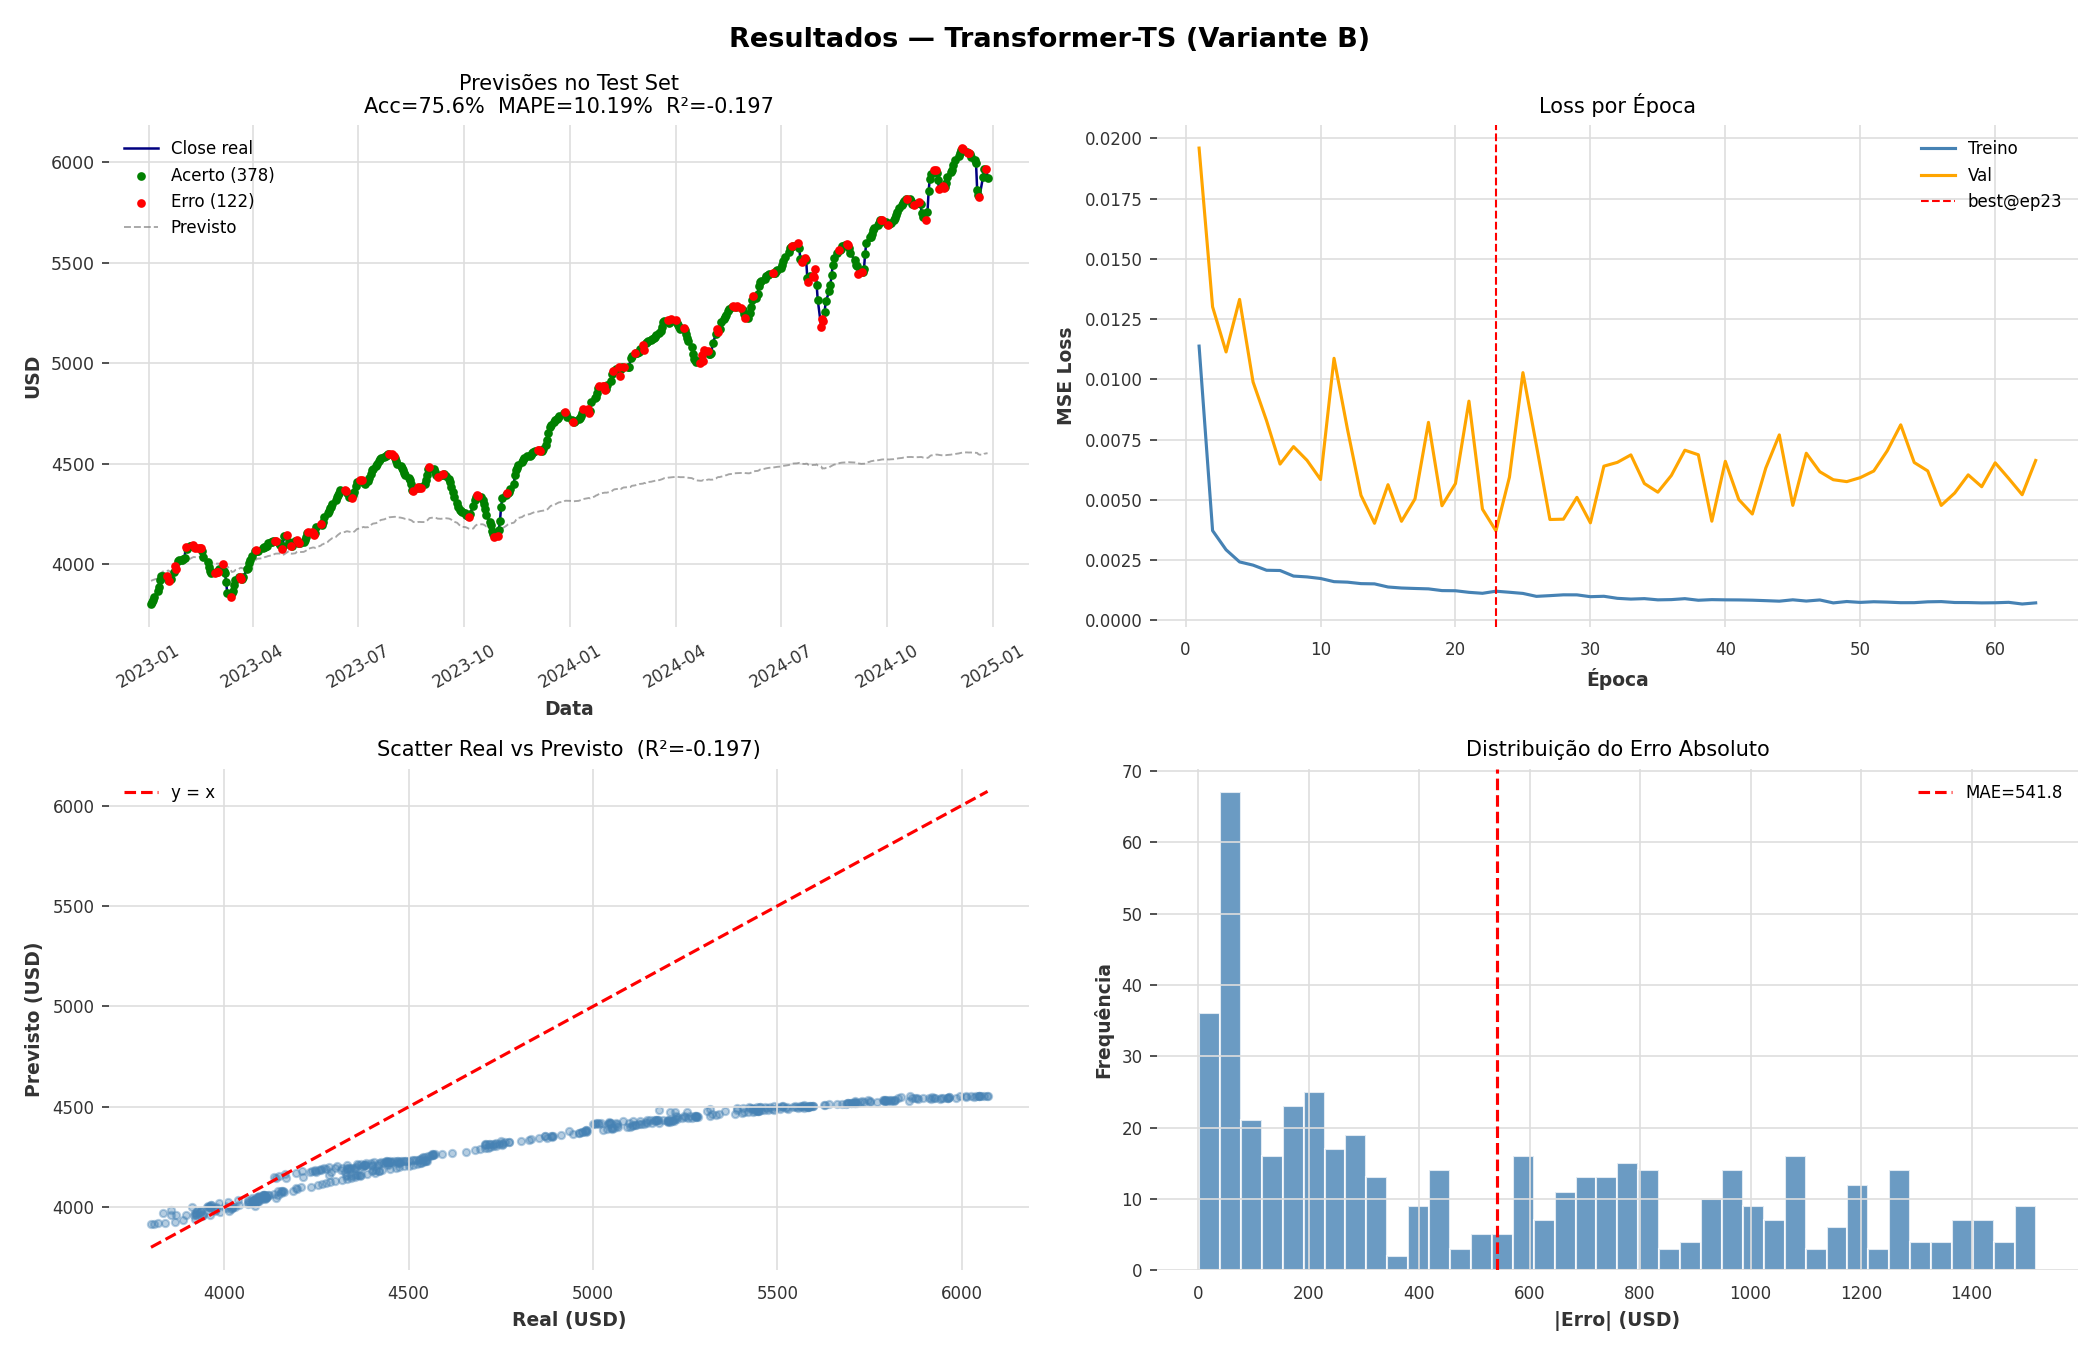
\includegraphics[width=\textwidth]{figuras/transformer_ts_resultados.png}
    \caption{Resultados do Transformer-TS no conjunto de teste (2023--2024).}
    \label{fig:transformer_resultados}
\end{figure}

\section{Comparativo Final das Três Arquiteturas}
\label{sec:res_comparativo}

A Tabela~\ref{tab:comparativo} compara os três modelos pelas métricas direcionais comuns (Acurácia e F1), uma vez que a LSTM realiza classificação direta e os modelos SOTA realizam regressão com direção derivada, tornando as demais métricas não comparáveis entre si. Cabe ressaltar que não foram aplicados testes estatísticos (como McNemar) para comparar o desempenho entre LSTM baseline e os modelos SOTA, pois estes últimos não foram treinados como classificadores direcionais, mas sim como regressores de valor absoluto com direção derivada em pós-processamento. Portanto, as comparações entre os três modelos são apresentadas de forma descritiva, com base nas métricas de acurácia e F1 derivadas.

\begin{table}[H]
\centering
\caption{Comparativo de acurácia e F1 direcional dos três modelos no conjunto de teste.}
\label{tab:comparativo}
\begin{tabular}{@{}lcc@{}}
\toprule
\textbf{Modelo} & \textbf{Acc (\%)} & \textbf{F1 (\%)} \\
\midrule
LSTM Var.~B    & 67,5 & 72,0 \\
xLSTM-TS       & 75,8 & 79,8 \\
Transformer-TS & 75,6 & 81,6 \\
\bottomrule
\end{tabular}
\end{table}


\section{Análise de Interpretabilidade SHAP}
\label{sec:res_shap}

O objetivo da análise SHAP (\textit{SHapley Additive exPlanations}) é identificar em quais pontos da janela de entrada cada modelo concentra sua atenção, quantificando a contribuição de cada passo temporal para a previsão. O SHAP atribui a cada \textit{timestep} um valor que representa sua contribuição na previsão em cada amostra. Como são avaliadas múltiplas amostras do conjunto de teste, a importância exibida nos gráficos é a média absoluta desses valores pelo número de amostras analisadas. Isso permite analisar o comportamento médio do modelo ao longo do período de teste.

Para a LSTM (janela de 20 dias, 18 \textit{features}), os valores SHAP são agregados pela média absoluta ao longo das \textit{features} e das amostras, resultando em um perfil de importância por posição da janela. Portanto, a análise revela em quais dos 20 dias da janela o modelo se apoia. Para o xLSTM-TS e o Transformer-TS (janela de 150 dias, 1 \textit{feature}), a importância por \textit{timestep} é direta, sem necessidade de agregação adicional.

A análise foi executada sobre 200 amostras do conjunto de teste (2023--2024). Cada ``amostra'' corresponde a uma janela de entrada completa (20 dias para a LSTM, 150 dias para os modelos SOTA) e sua respectiva previsão. O SHAP calcula valores individuais para cada amostra; os gráficos exibem a média absoluta desses valores sobre as 200 amostras analisadas.

As Figuras~\ref{fig:shap_lstm}, \ref{fig:shap_xlstm} e~\ref{fig:shap_transformer} apresentam os quatro painéis para a LSTM, o xLSTM-TS e o Transformer-TS, respectivamente. Cada figura desta seção é composta por quatro painéis complementares. Painel superior esquerdo: importância média por posição da janela, mostrando a distribuição de atenção ao longo dos \textit{timesteps}. Para a LSTM, o gráfico é exibido como barras (janela menor, 20 dias), enquanto para os modelos SOTA, exibido como linha (janela maior, 150 dias), porém ambos representam a mesma informação. Painel superior direito: heatmap da magnitude da contribuição (\textbar SHAP\textbar) por amostra de teste; o eixo horizontal representa cada uma das 200 amostras, o eixo vertical representa os \textit{timesteps} da janela (0 = mais antigo) e a cor indica a intensidade da influência (cor amarela = maior importância, cor roxa = importância próxima a zero). Painel inferior esquerdo: \textit{ranking} dos 10 \textit{timesteps} mais influentes. Painel inferior direito: curva de Pareto da importância acumulada, indicando quantos \textit{timesteps} são necessários para explicar 90\% da importância total (quanto mais íngreme a curva, mais concentrada é a atenção do modelo).



\begin{figure}[H]
    \centering
    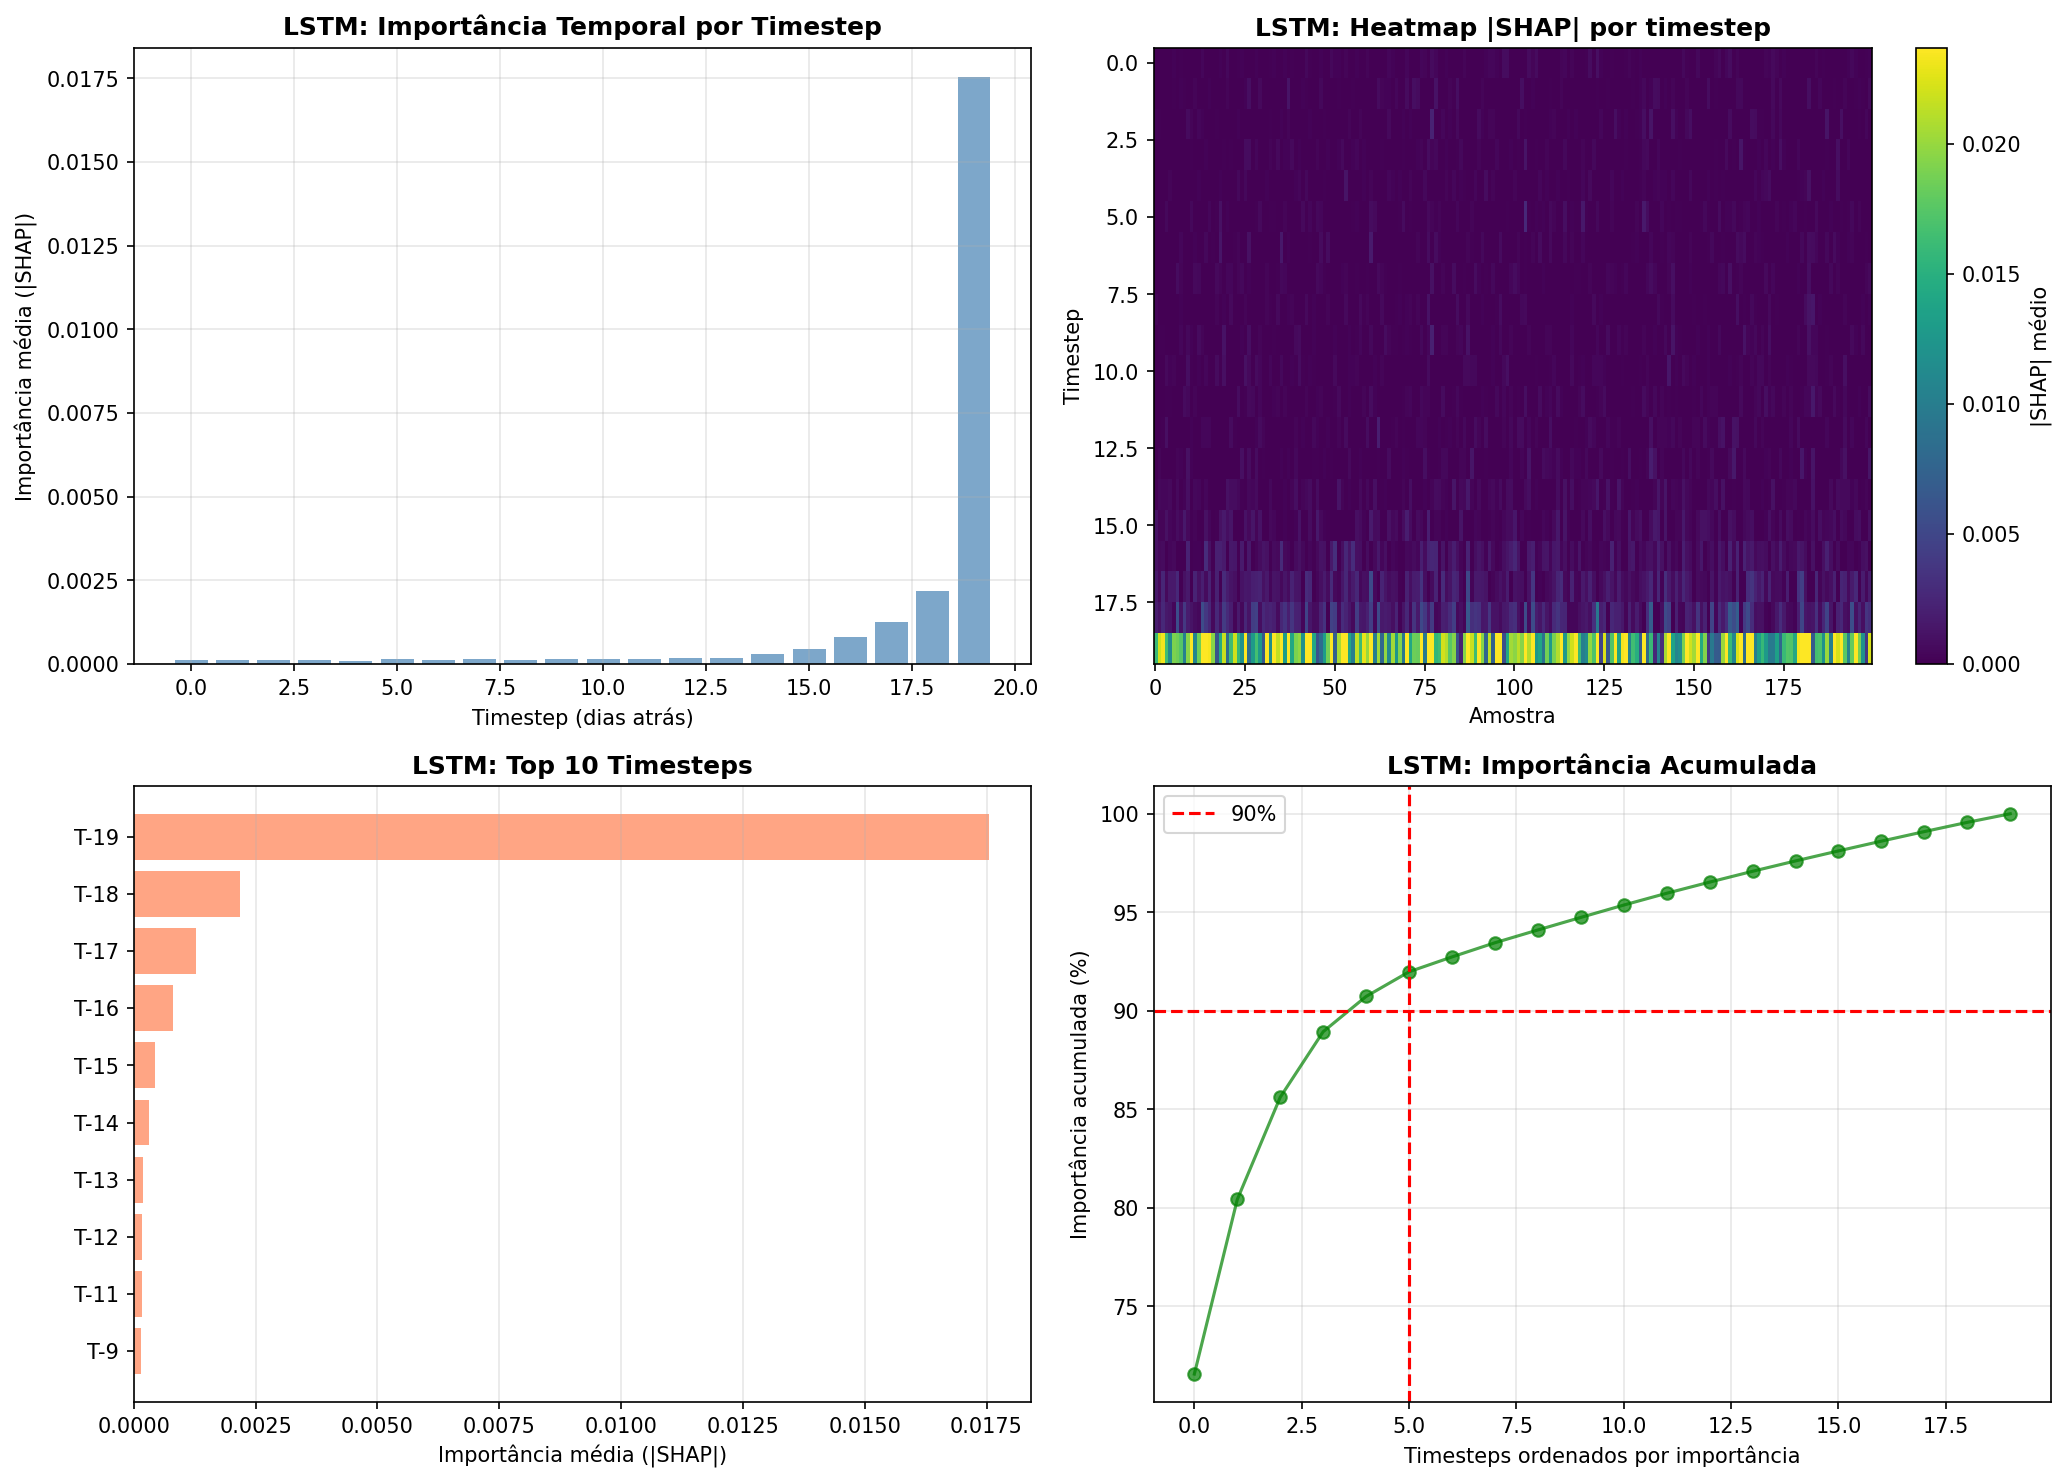
\includegraphics[width=0.85\textwidth]{figuras/shap_lstm.png}
    \caption{Análise SHAP da LSTM (Variante~B) sobre 200 amostras do conjunto de teste (2023--2024).}
    \label{fig:shap_lstm}
\end{figure}

\begin{figure}[H]
    \centering
    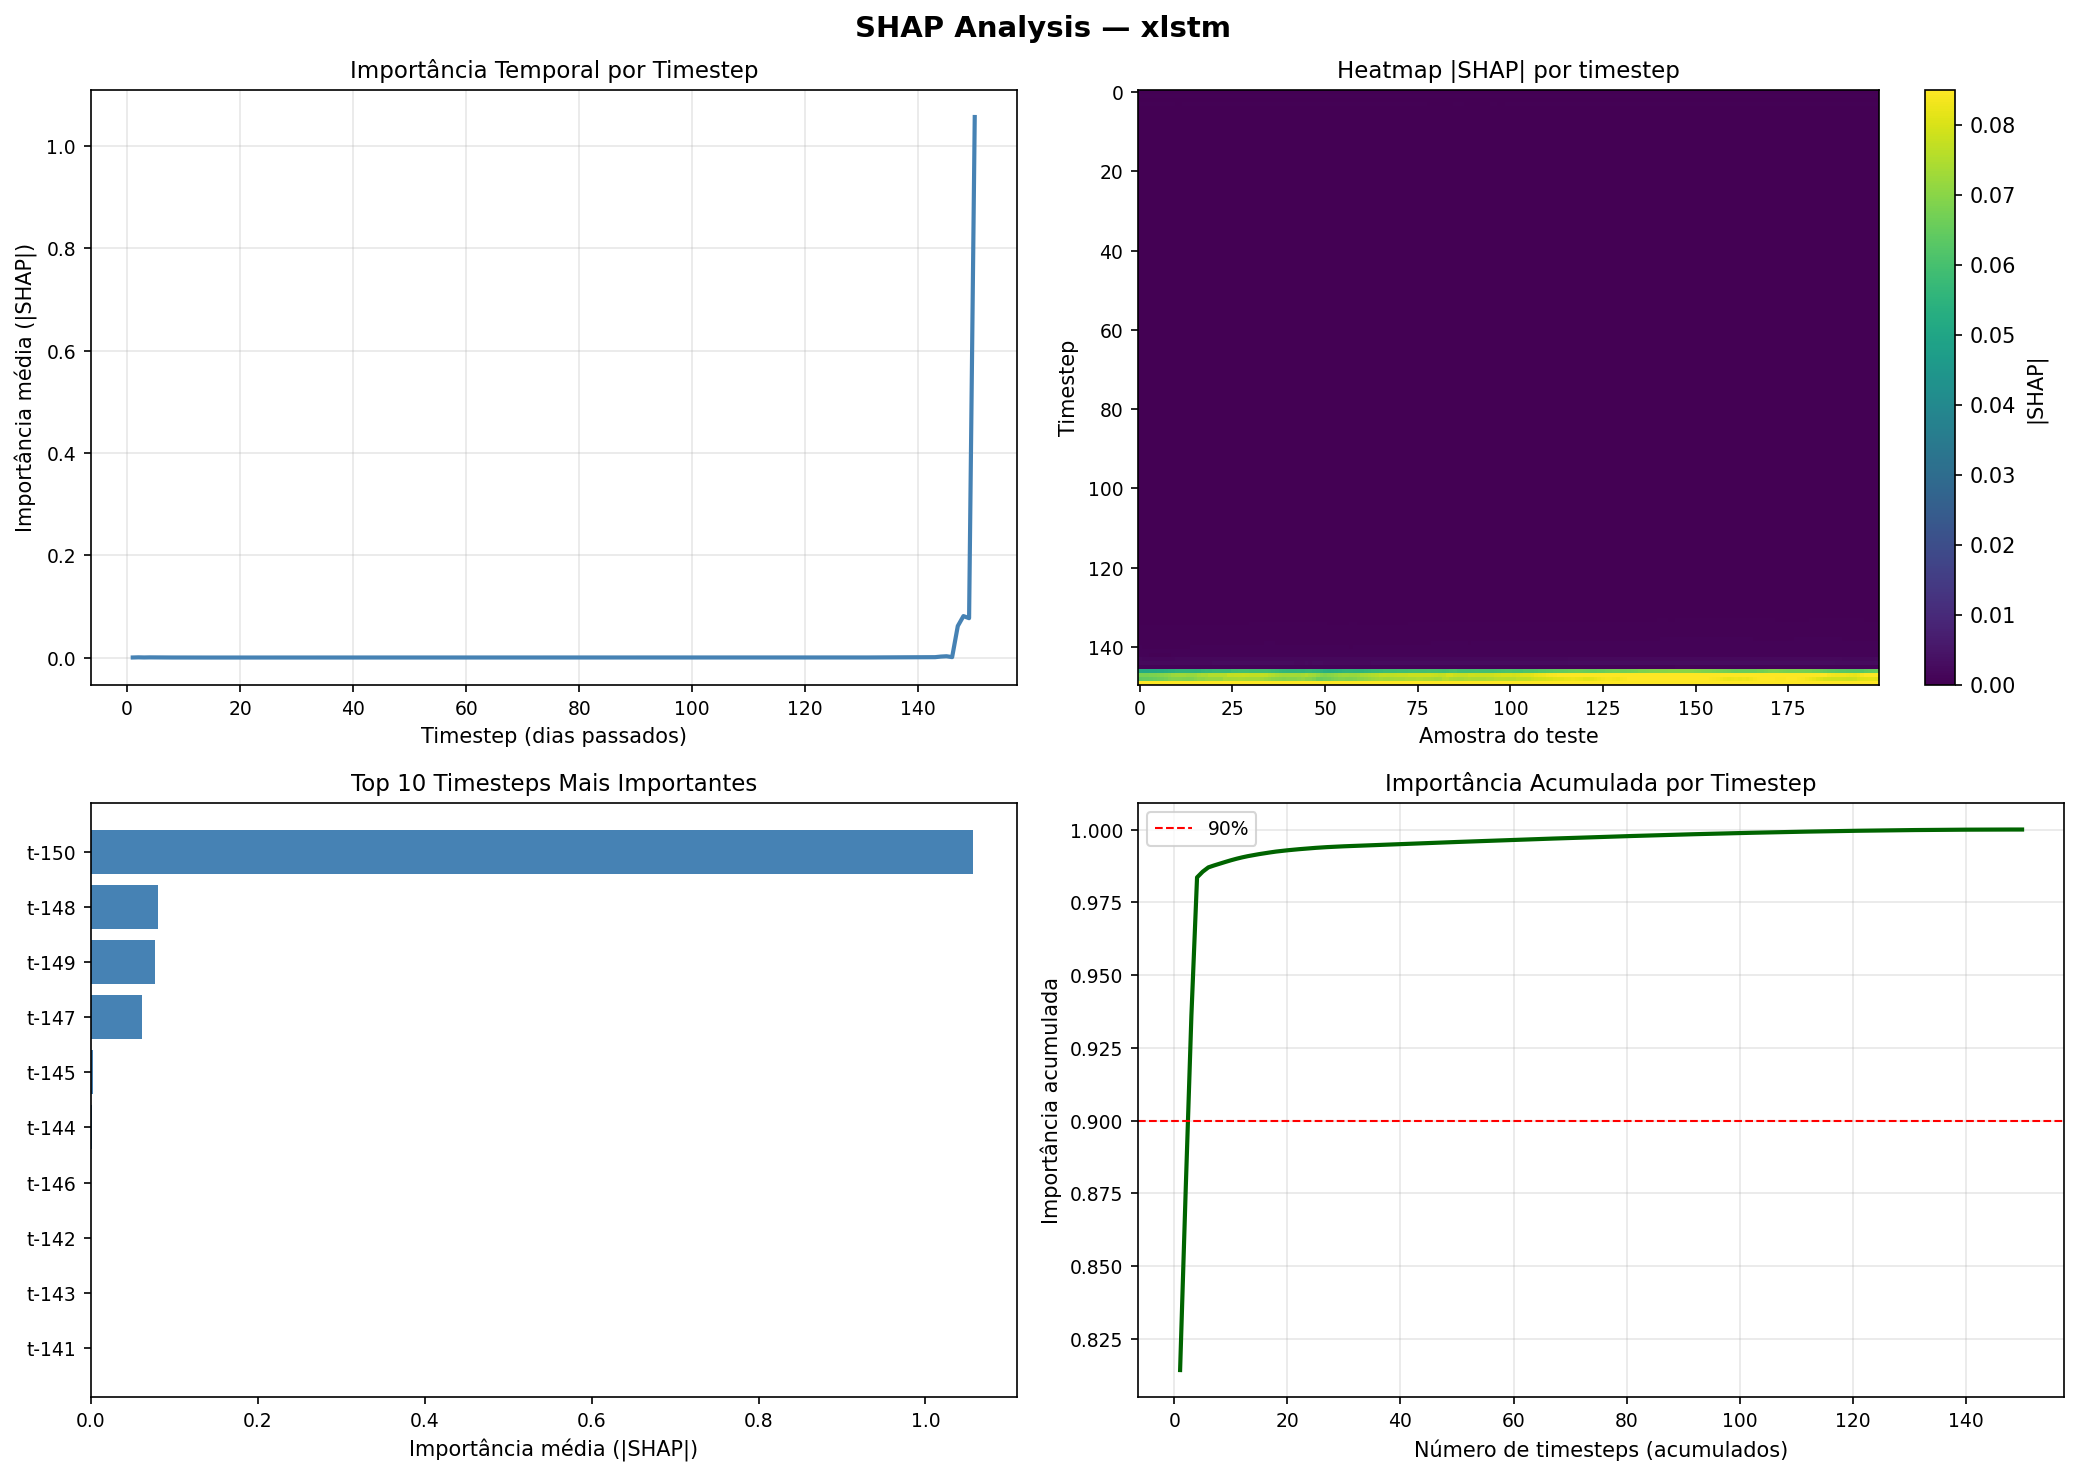
\includegraphics[width=0.85\textwidth]{figuras/shap_xlstm.png}
    \caption{Análise SHAP do xLSTM-TS no conjunto de teste (2023--2024).}
    \label{fig:shap_xlstm}
\end{figure}

\begin{figure}[H]
    \centering
    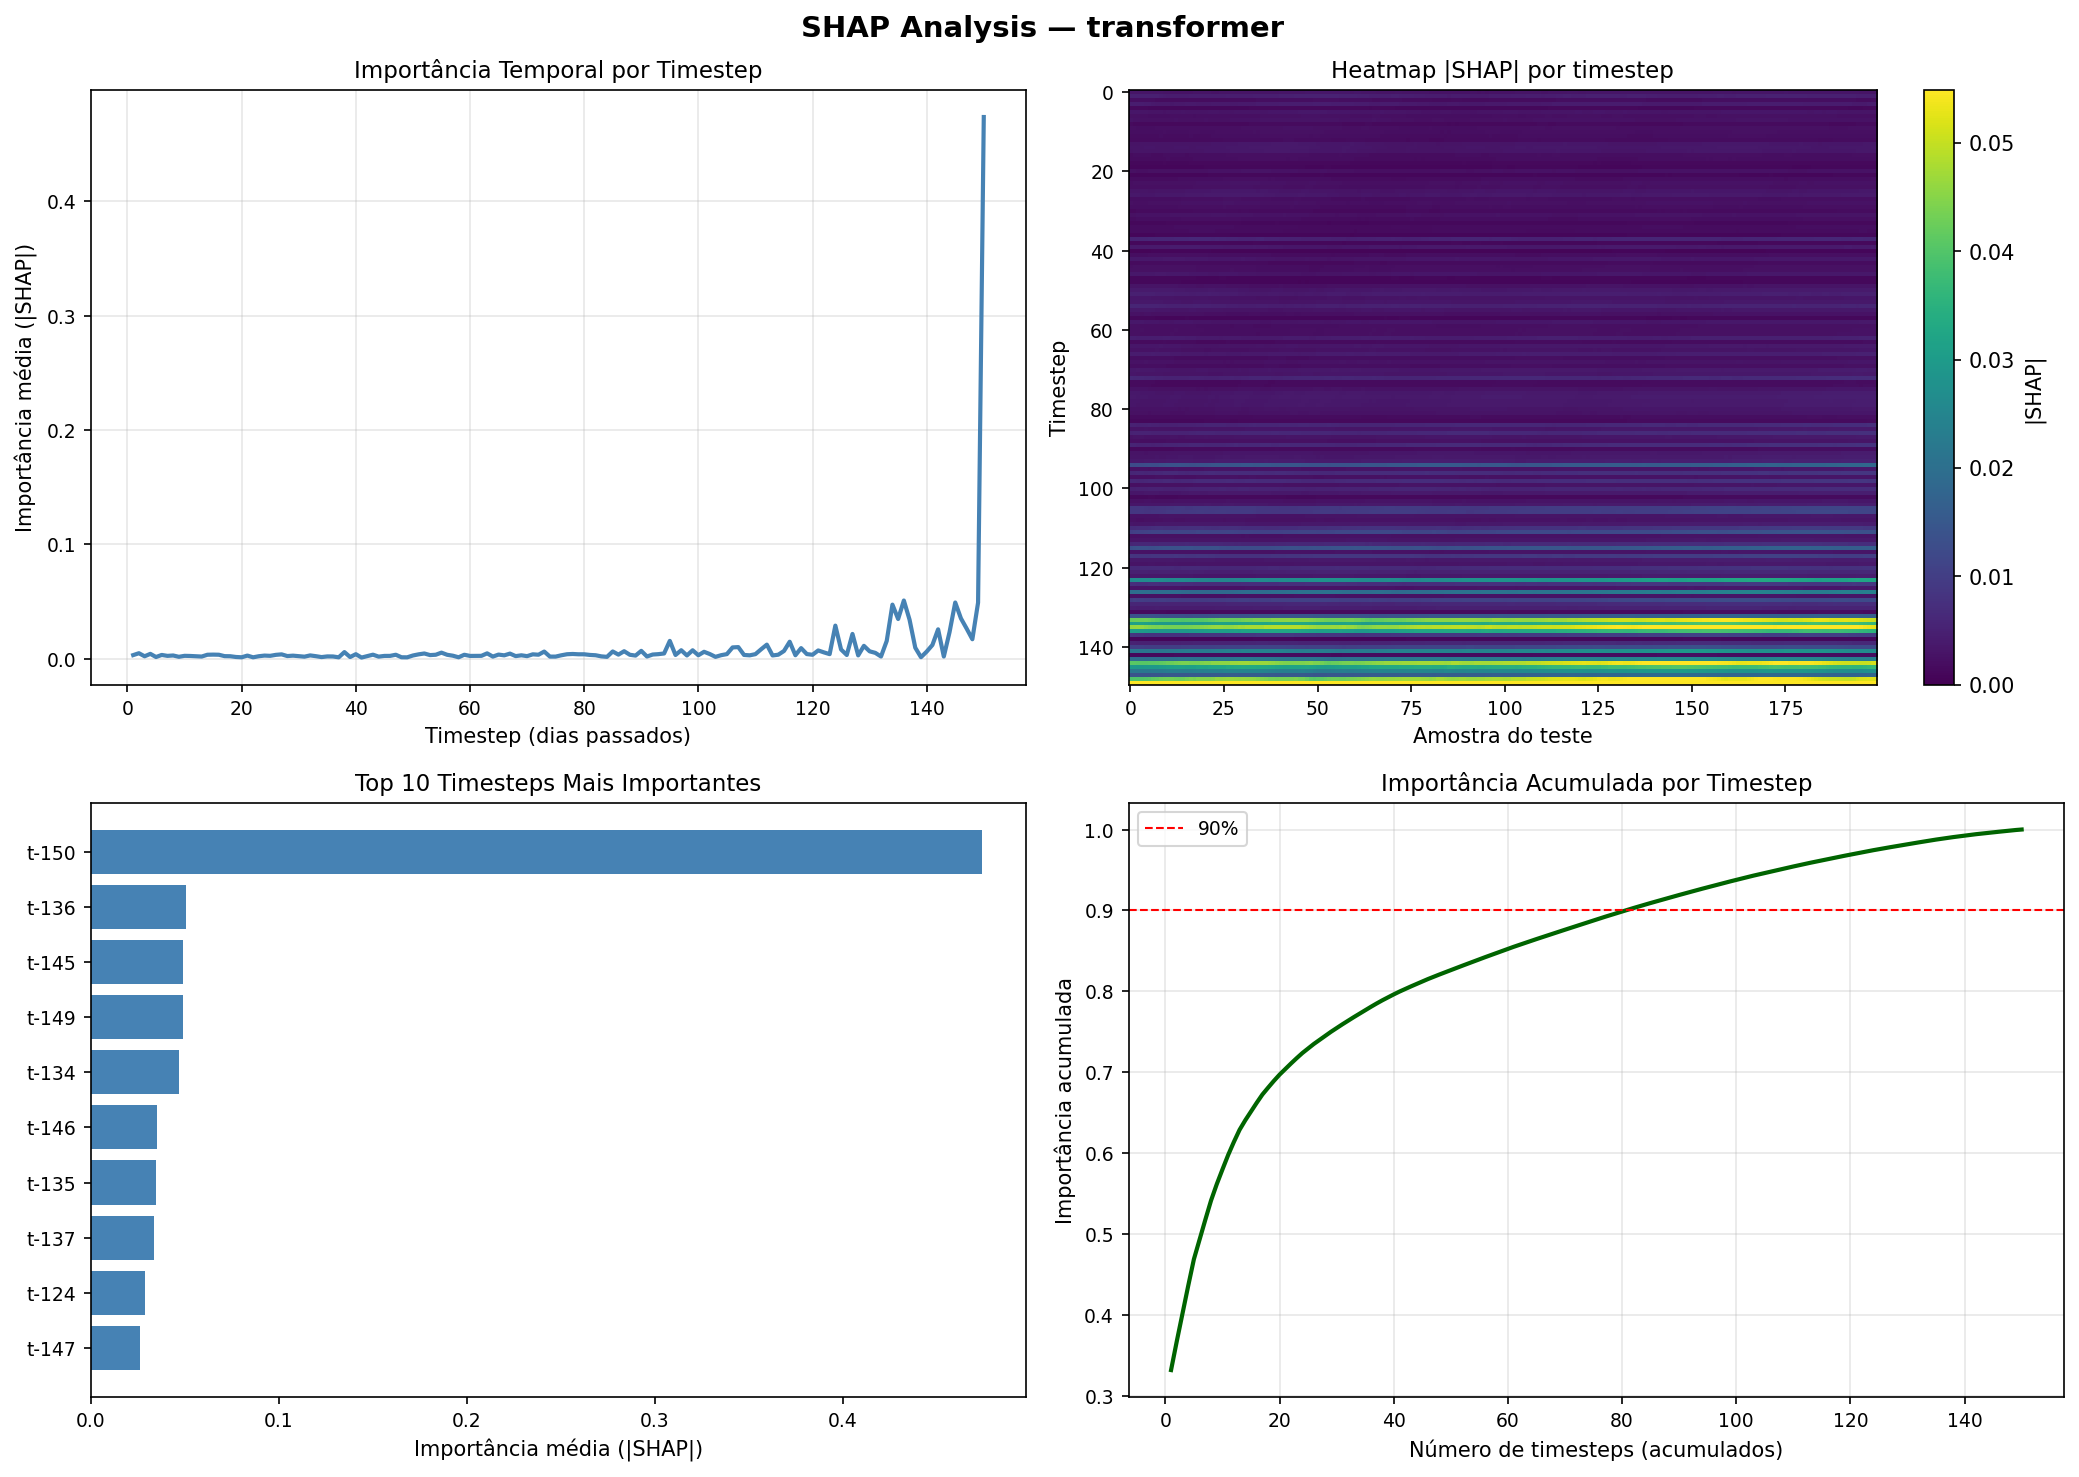
\includegraphics[width=0.85\textwidth]{figuras/shap_transformer.png}
    \caption{Análise SHAP do Transformer-TS no conjunto de teste (2023--2024).}
    \label{fig:shap_transformer}
\end{figure}
